En el año dos mil cuatro, el por aquel entonces estudiante de esta universidad, 
Iván Castilla Rodríguez - y ahora tutor de este trabajo de fin de grado-, 
desarrolló como proyecto final de carrera un Simulador didáctico para la enseñanza 
de arquitectura de computadores, el cual fue bautizado como Simde. \cite{SIMDE}

\bigskip
Este simulador como se ha comentado en el apartado 1.4 cumple con las características
deseadas y esperadas de un simulador para la docencia de este ámbito.

\bigskip
Sin embargo, esta herramienta ya se encuentra desfasada. No ha sido un proyecto en constante
evolución, fue diseñada utilizando C++98 y C++ Builder y el código ahora mismo no resultaría
fácil de adaptar y mantener.

\begin{figure}[!th]
\begin{center}
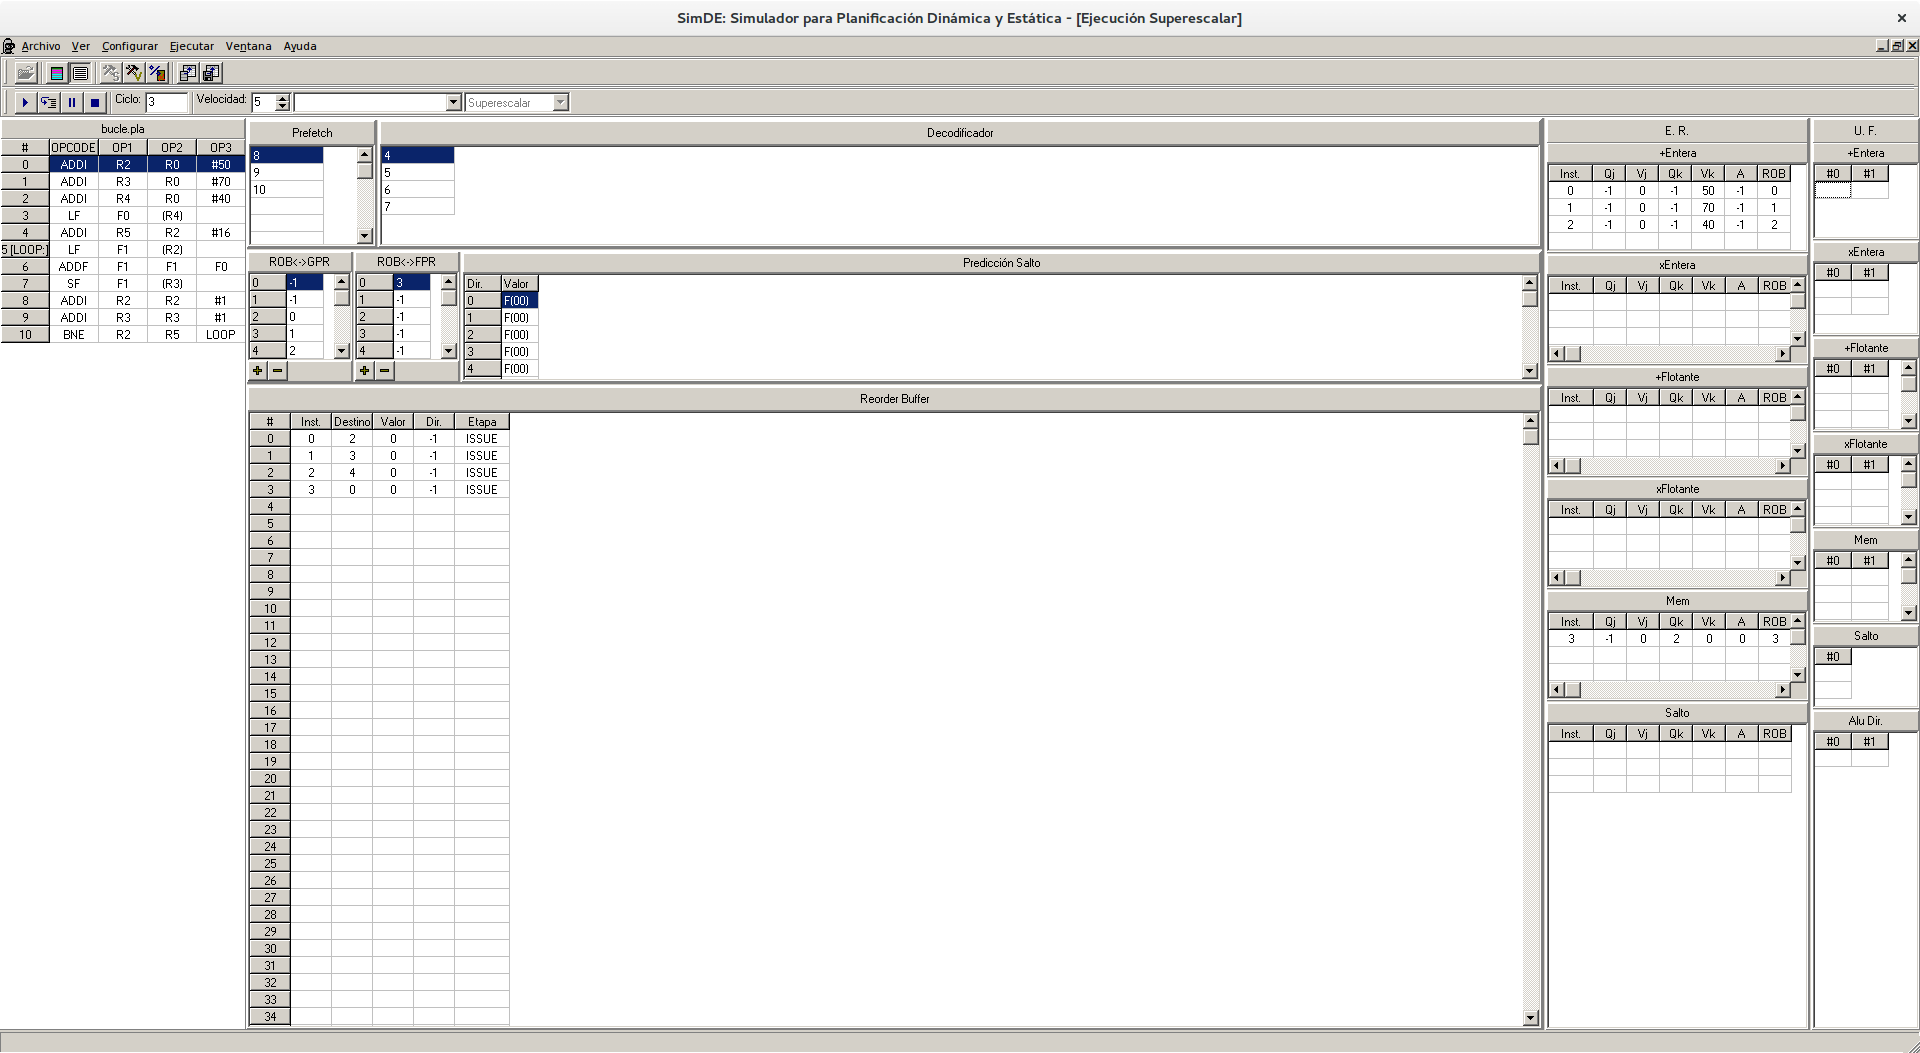
\includegraphics[width=0.8\textwidth]{images/cap2/simdeoriginal.eps}
\caption{Simulador original SIMDE}
\label{fig:Simulador original SIMDE}
\end{center}
\end{figure}